\section{Evaluation} \label{sec-evaluation} 
In this section, we evaluate the performance of our platform.
We evaluate both the performance improvement with regards to reduction in time and increase in overall model quality.

\subsection{Hyperparameter Tuning}
\todo[inline]{These results are still without the 'Avoiding Local Optima' solution, so ideally, once we find a good solution to avoid local optimas we should get even better results.}
Figure \ref{fig-avg-warm-vs-cold-task-31} shows the result of bayesian optimization on a machine learning pipeline from OpenML database.
The specified task\footnote{https://www.openml.org/t/31} relates to the classification of customers as good or bad credit risks using the German Credit data from he UCI repository \cite{Dua:2017}.
\todo[inline]{include other pipeline ids when the experiment is finalized}
In this experiment we focus on several of the popular machine learning pipelines (flow 7707\footnote{https://www.openml.org/f/7707}) designed for solving this task.
We extracted the meta-data from the OpenML database which includes all the executions of the pipeline, the value of the hyperparameters, and the evaluation metrics.
Using the meta-data, we initialize the bayesian search optimization procedure, with the values of the hyperparameters for each execution and the loss ($1- accuracy$) for the specific execution.
We then execute the bayesian optimization with a budget of 100 trials, trying to minimize the loss of the openml pipeline.
We repeat this experiment 10 times.
Figure \ref{fig-avg-warm-vs-cold-task-31} shows the average of losses of the 100 trials for the 10 experiments for several pipelines from openml.
Warmstarting the search decreases the overall loss of the trials.
On average, warmstarting decreases the error rate from 0.25 to 0.21.
\begin{figure}
\centering
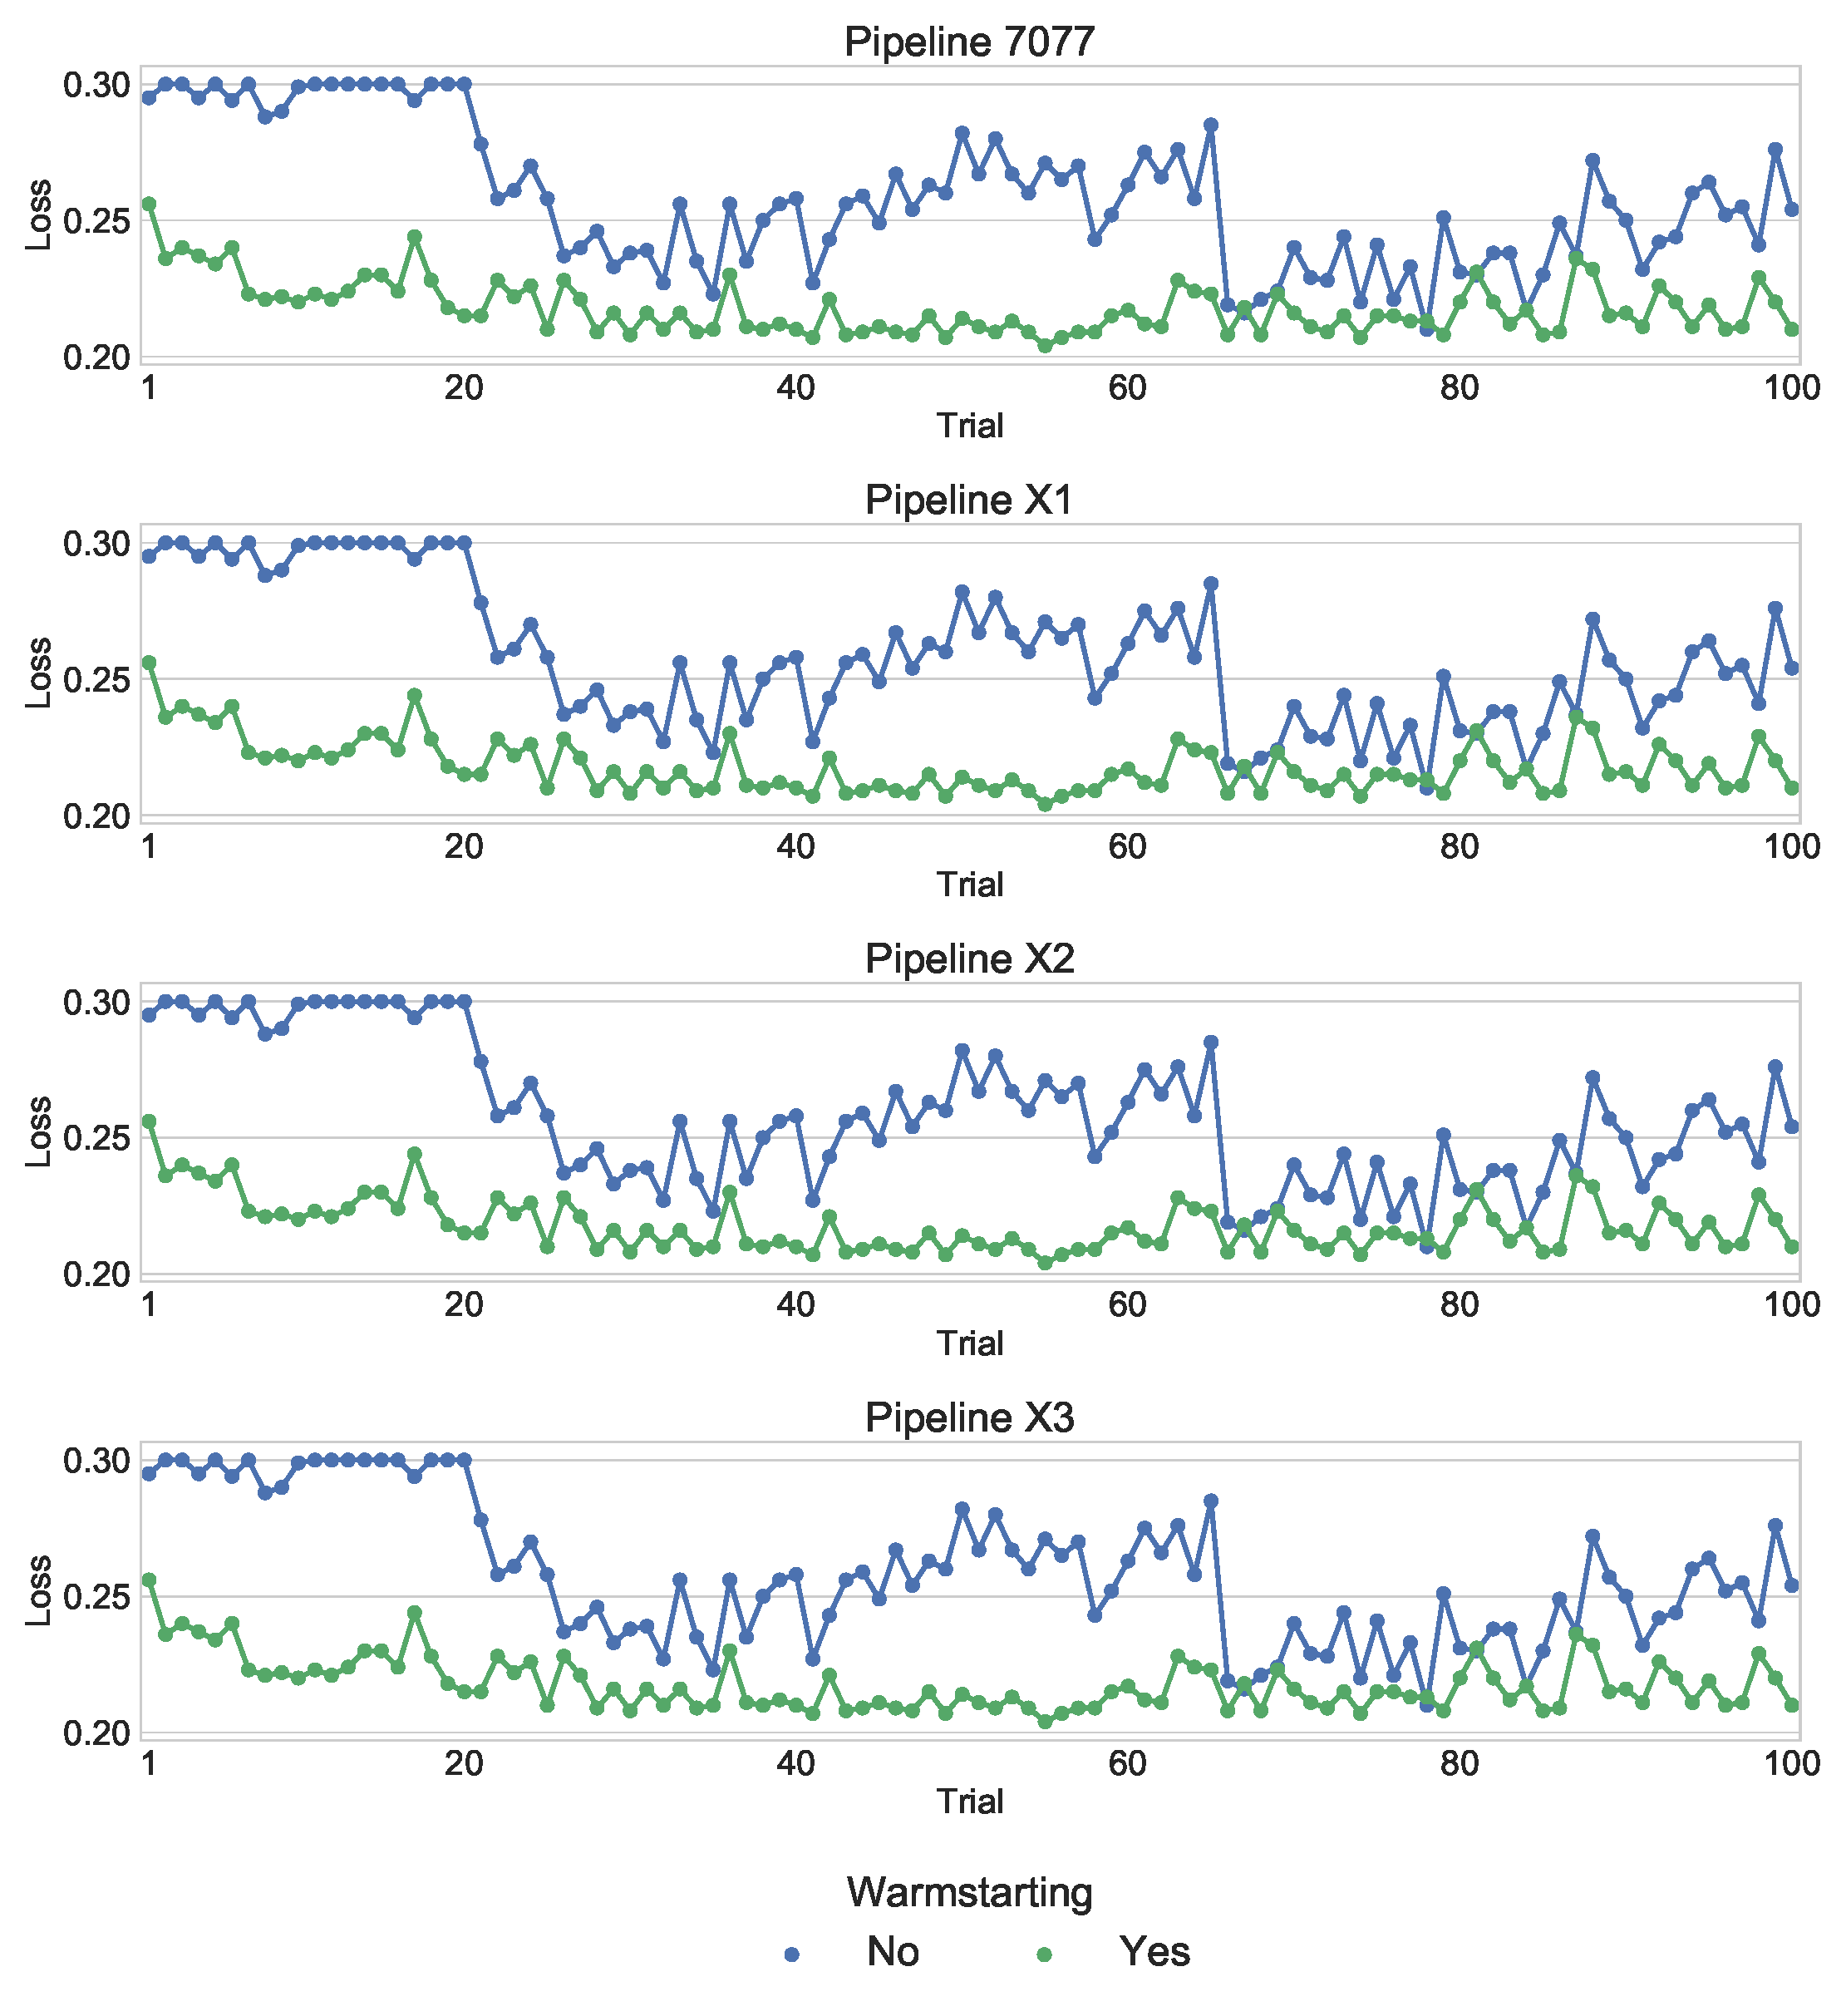
\includegraphics[width=\columnwidth]{../images/experiment-results/task31-cold-starting-warm-avgtrials.eps}
\caption{Loss value of 100 Trials with and without warmstarting}
\label{fig-avg-warm-vs-cold-task-31}
\end{figure}

Table \ref{table-best-hyperparameters} shows the best loss achieved from the search process for every pipeline on the Task 31.
Figure \ref{figure-best-hyperparameters} shows the number of time that the search process (with budget of 100) manages to find the best set of hyperparameters that results in the lowest loss value.
While both with and without warm starting does find the best set of hyperparameters, using warmstarting outperforms the search without wamrstarting and has a higher probability of finding the best hyperparameters.

\begin{minipage}{\columnwidth}
  \begin{minipage}[m]{0.49\columnwidth}
   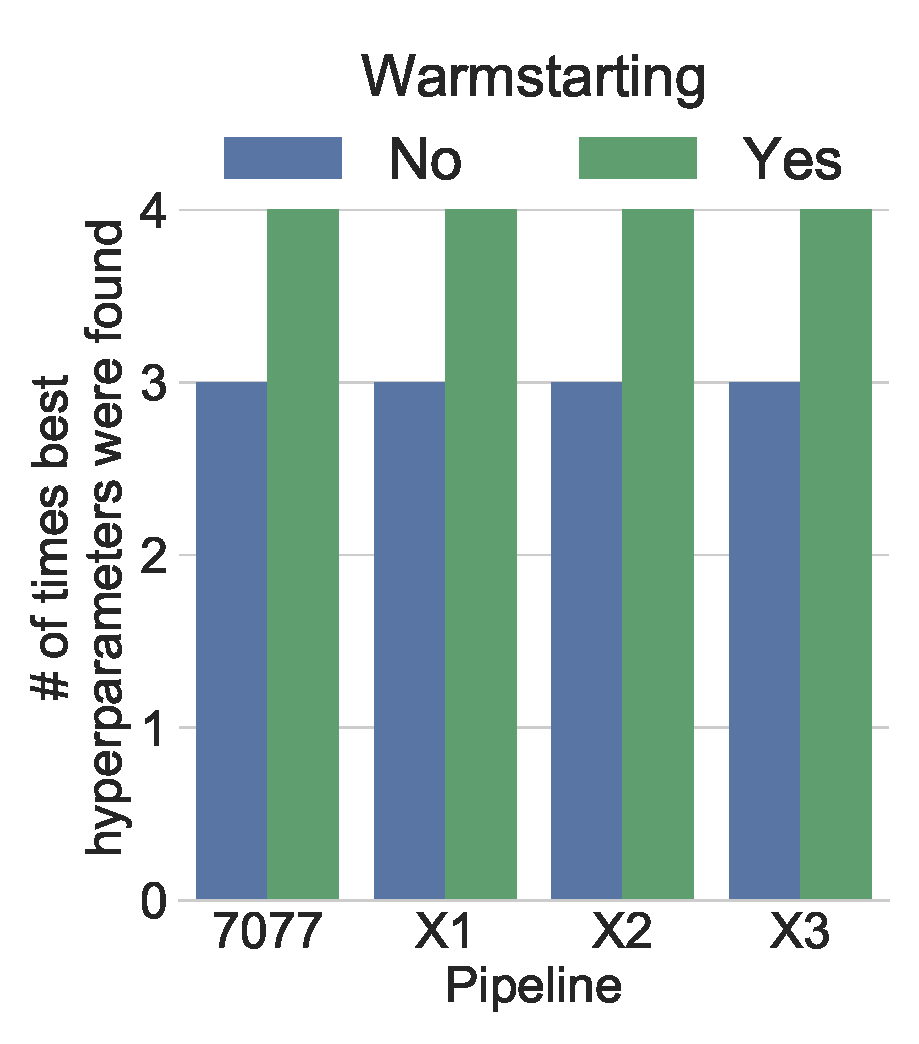
\includegraphics[width=\columnwidth]{../images/experiment-results/task31-cold-starting-warm-besthyperparametersfound.eps}
    \captionof{figure}{Occurrences of best hyperparameters}
     \label{figure-best-hyperparameters}
  \end{minipage}
  \hspace{0.5cm}
  \begin{minipage}[m]{0.49\columnwidth}
    \begin{tabular}{cc}\hline
      Pipeline & Best Loss \\ \hline
        7077 & 0.189 \\
        X1 & XXX \\
        X2 & XXX \\
        X3 & XXX\\ \hline
      \end{tabular}
      \captionof{table}{Best hyperparameters}
      \label{table-best-hyperparameters}
    \end{minipage}
  \end{minipage}
\subsection{Data Materialization}